\section{Singleton}

The singleton pattern is a software design pattern that restricts the instantiation of a class to one object. This is useful when exactly one object is needed to coordinate actions across the system. The pattern involves a single class which creates an object like while making sure that only single object is created.

\subsection*{Example}

% Description of the roles of the class in the design pattern
Figure~\ref{fig:singleton} presents the UML diagram for the singleton design pattern found in the project \textit{ObjectExplorer}.

\begin{figure}[htb]
    \centering
    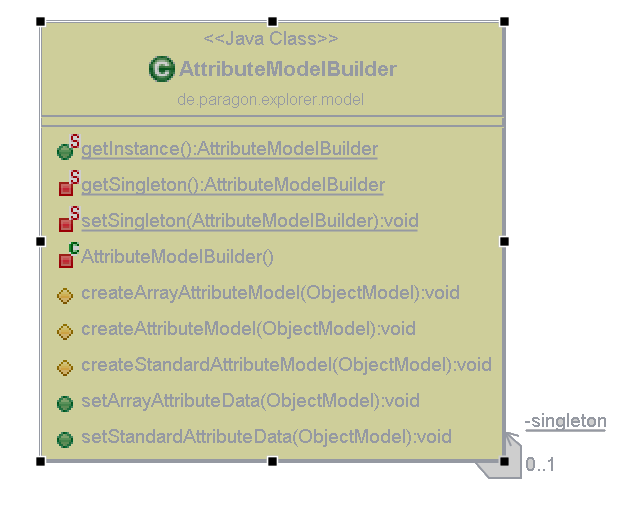
\includegraphics[width=9cm]{images/Singleton.png}
    \caption{Singleton design pattern in the project \textit{ObjectExplorer}}
    \label{fig:singleton}
\end{figure}
\FloatBarrier

Figure~\ref{fig:AttributeModelBuilder} presents the class \texttt{AttributeModelBuilder}. We can see the instance receiving the instance of an Object and we can see how it obtains a single object.

\begin{figure}[htb]
\centering
\lstset{language=Java, basicstyle=\scriptsize, stepnumber=1, showspaces=false, showstringspaces=false,breaklines=true}
\begin{lstlisting}
 static {
         public final class AttributeModelBuilder {
	private static AttributeModelBuilder	singleton;

	public static AttributeModelBuilder getInstance() {
		return AttributeModelBuilder.getSingleton();
	}
	private static AttributeModelBuilder getSingleton() {
		if (AttributeModelBuilder.singleton == null) {
			AttributeModelBuilder.setSingleton(new AttributeModelBuilder());
		}
		return AttributeModelBuilder.singleton;
	}
		private static void setSingleton(AttributeModelBuilder builder) {
		AttributeModelBuilder.singleton = builder;
	}
}
                }
             }
          );
 }
\end{lstlisting}
\caption{[Singleton] AttributeModelBuilder.java}
\label{fig:AttributeModelBuilder}
\end{figure}
\FloatBarrier
